\newcommand{\imagewidth}{0.8\textwidth}

In this chapter we introduce briefly the main notions required to appreciate this work.

\section{The mathematical mesh model}

Meshes often model physical objects and phenomena. This is typically achieved through the discretization of a continuous model, such as the surface or volume of an object, in order to approximate its physical properties to a desired degree of precision.
\par

The mesh model consists of a hierarchy of elements, which may include a subset the following:
\begin{itemize}
\item Polyhedra such as cubes or tetrahedrons
\item Polygons \emph{(also referred to as cells or faces)} such as triangles and quadrilaterals
\item Edges
\item Vertices \emph{(also referred to as nodes)}
\end{itemize}

\includesvg[width=\imagewidth, svgpath=images/background/]{mesh-elements}

Each element in the above hierarchy is built-up from those below it. Thus, a polyhedron is assimilated by a set of polygons, a polygon is composed by a set of edges, and an edge joins two vertices.


\subsection{Geometry vs topology}
There is a key distinction to make between the geometric and topological properties of a mesh.

Since meshes model a physical reality, the elements of a mesh may be spatially embedded: vertices are associated with points in space, and edges are formed as segments joining their two vertices. This affects \emph{geometric} properties of the mesh, such as its surface area or volume.

On the other hand, the hierarchy of elements described above induces a mesh topology. This describes the connectedness of the mesh, that is to say how elements relate to one another. For instance, we may describe two vertices sharing an edge as \emph{adjacent}, or two cells being \emph{incident} on an edge.
\par
In this work we concern ourselves solely with the topological structure of meshes, treating its geometry as arbitrary data that is associated with its respective elements (the position of a vertex for instance). Figure~\ref{fig:same-topology} illustrates the difference between the two concepts.

\begin{figure}
    \includesvg[width=\imagewidth, svgpath=images/background/]{same-topology}
    \caption{Despite having completely different geometric shapes and properties, the two meshes are topologically equivalent. The labels indicate corresponding vertices.}
    \label{fig:same-topology}
\end{figure}




\subsection{Manifold meshes}
A mesh is a manifold if the following properties hold:
\begin{enumerate}
\item All edges are adjacent to either one or two faces.

\item All faces meeting at a given vertex must form either an open or a closed fan around that vertex (Figure~\ref{fig:open-closed-fans}).
\end{enumerate}

% Open and closed fans
\begin{figure}
    \sidebyside
        {\includesvg[width=\imagewidth, svgpath=images/background/]{closed-fan}
        \caption{A closed fan}}
        {\includesvg[width=\imagewidth, svgpath=images/background/]{open-fan}
        \caption{An open fan}}
    \caption{}
    \label{fig:open-closed-fans}
\end{figure}

Figure~\ref{fig:non-manifolds} demonstrates examples of non-manifold meshes. In this work we consider manifold meshes exclusively, and future mentions of `mesh' shall implicitly refer to manifold meshes.

% Non-manifolds
\begin{figure}
    \sidebysidefour
    {\includesvg[width=\imagewidth, svgpath=images/background/]{bad-fan}
        \caption{Faces incident on a vertex which do not form a continuous fan}}
    {\includesvg[width=\imagewidth, svgpath=images/background/]{bad-fan2}
        \caption{An extra face that breaks off from the otherwise closed fan}}
    {\includesvg[width=\imagewidth, svgpath=images/background/]{bad-multi-edge}
        \caption{More than two faces incident on a single edge}}
    {\includesvg[width=\imagewidth, svgpath=images/background/]{bad-no-edge}
        \caption{An edge with no incident faces}}

    \caption{Examples of non-manifold meshes.}
    \label{fig:non-manifolds}
\end{figure}





\section{The mesh data structure}

We describe how a mesh model is manifest at the data structure level. There are three general component types can be identified:
\begin{itemize}
\item Entity sets
\item Associative data
\item Relations between two entity sets
\end{itemize}

In the following sections, the examples shall refer to the mesh depicted in figure~\ref{fig:example-mesh}.

\begin{figure}
    \includesvg[width=\imagewidth, svgpath=images/background/]{mesh-data-structure}
    \caption{Example mesh with labelled elements.}
    \label{fig:example-mesh}
\end{figure}


\subsection{Entity sets}
Each set represents a certain type of entity in the mesh, such as vertices or cells. Each element in a set is associated with a unique identifier. Integers are a common choice as an identifier for a couple of reasons:
\begin{itemize}
\item They need not be enumerated explicitly. All we need is the set cardinality and a starting index.
\item They are convenient for direct-indexed array accesses, as well as for more general indexing methods.
\end{itemize}

See figure~\ref{fig:entity-sets} for examples.

\begin{figure}
    \includesvg[width=\imagewidth, svgpath=images/background/]{entity-sets}
    \caption{The entity sets of the mesh in figure~\ref{fig:example-mesh}. These are (from left to right) the vertices, edges, and cells.}
    \label{fig:entity-sets}
\end{figure}


\subsection{Associative data}
Arbitrary data which is associated with elements of a particular entity set. For instance, spatial coordinates associated with each vertex. A typical representation is a flat array indexed by element identifier.
This is the data over which we perform our computations and ultimately care about. Everything else is incidental.
See figure~\ref{fig:associative-data} for an example.

\begin{figure}
    \includesvg[width=\imagewidth, svgpath=images/background/]{associative-data}
    \caption{Coordinate data associated with the vertices of the mesh in figure~\ref{fig:example-mesh}.}
    \label{fig:associative-data}
\end{figure}


\subsection{Relation maps between two entity sets}
Entity sets may have relations defined between them, a mapping from an element in a source set to one or more corresponding elements in the destination set. For instance, we may have an adjacency relation from the vertex set to itself, or an inclusion relation from the cell set to the vertex set.
In a general unstructured mesh these relations must be explicitly stored, typically as an array indexed by the source element's identifier.
See figure~\ref{fig:relation} for an example.

\begin{figure}
    \includesvg[width=\imagewidth, svgpath=images/background/]{relation}
    \caption{Inclusion relation from cells to vertices, as depicted in the mesh of figure~\ref{fig:example-mesh}.}
    \label{fig:relation}
\end{figure}




\section{The core-computation contract}
Given a mesh model and its underlying representation, computation logic provided by an external user is to be executed. We refer to this as the \emph{core-computation} so as to disambiguate it from other incidental processing, such as structure detection.
Our contract to the user is described in what follows.

\subsection{Given: operating set}
We are given an entity set over which to operate, for example the set of edges or the set of cells. We refer to this entity set as the \emph{operating set}. The core-computation consists of executing a computation for each element of the operating set. This is analogous to the \emph{map} phase of the MapReduce programming model\footnote{REFERENCE}, though we restrict our usage of the term \emph{map} to refer to relation maps.

\subsection{Given: relation-map tree}
We are given a tree structure defining which relation maps to use and how to access them. This is best explained through an example, illustrated in figure~\ref{fig:relation-tree}. The core-computation will, for each element in the operating set, gather all indexing variables as described by the relation-map tree.


\begin{figure}
    %% Key icon
    \newcommand{\keyicon}{\includesvg[width=6pt, svgpath=images/background/]{key}}

    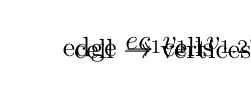
\begin{tikzpicture}[every tree node/.style={draw,circle},
        level distance=1.5cm,
        edge from parent path={(\tikzparentnode) -- (\tikzchildnode)}]

    \tikzset{level 2/.style={sibling distance=0.8cm}}

    \Tree
    [.{$e$}
        \edge node[auto=right] {\keyicon};
        [.\node[rectangle] {edge $\rightarrow$ cells};
            [.{$c_1$}
                \edge node[auto=right] {\keyicon};
                [.\node[rectangle] {cell $\rightarrow$ vertices};
                    [.$v_{1.1}$ ]
                    [.$v_{1.2}$ ]
                    [.$v_{1.3}$ ]
                    [.$v_{1.4}$ ]
                ]
            ]
            [.{$c_2$}
                \edge node[auto=right] {\keyicon};
                [.\node[rectangle] {cell $\rightarrow$ vertices};
                    [.$v_{2.1}$ ]
                    [.$v_{2.2}$ ]
                    [.$v_{2.3}$ ]
                    [.$v_{2.4}$ ]
                ]
            ]
        ]
    ]
    \end{tikzpicture}
    \caption{
    In this example, we consider a core-computation operating over the edge set, with $e$ being the indexing variable into the edge set.
    The edge $\rightarrow$ cells map is indexed by $e$ to obtain the the two cells $c_1$ and $c_2$ incident on the edge $e$. The cell $\rightarrow$ vertices map is then indexed by both $c_1$ and $c_2$ to obtain their respective vertices. The key symbol denotes indexing into the map below, using the indexing variable above.
    }
    \label{fig:relation-tree}
\end{figure}


\subsection{Given: kernel function}
We are given a kernel function specifying the computation logic, which is applied to each element in the operating set. It takes as arguments all gathered indexing variables, and it has read and write access to the mesh's associated data.

The kernel function is applied to the operating set elements in no particular order; the indexing variables, however, are passed to the kernel in some known order.


\subsection{Expected operation}
Given all the above, a core-computation is then performed as follows:
\begin{enumerate}
\item Iterate over the elements of the operating set, in no particular order.
\item For each element iterated over:
    \begin{enumerate}
    \item Gather any indexing variables as defined by the relation-map tree. This may involve indexing variables obtained through a chain of relation-maps.
    \item Call the kernel function, passing the gathered indexing variables in some known order. The kernel function may access any associative data using these indexing variables.
    \end{enumerate}
\end{enumerate}
